\documentclass[10pt]{beamer}

\usetheme{metropolis}
\usecolortheme{beaver}
\usepackage{appendixnumberbeamer}

\usepackage{booktabs}
\usepackage[scale=2]{ccicons}

\usepackage{pgfplots}
\usepgfplotslibrary{dateplot}

\usepackage{xspace}
\newcommand{\themename}{\textbf{\textsc{metropolis}}\xspace}
\usepackage[brazil]{babel}  % AAB
\usepackage{bibentry}       % AAB
\usepackage{amsmath, bm}    % AAB
%\usepackage[utf8]{inputenc}                  % AAB inserido
                                              % AAB inserido
\usepackage[caption=false,font=normalsize,labelfont=sf,textfont=sf]{subfig}
%\usepackage[caption=false,font=footnotesize]{subfig}
%
\DeclareMathOperator{\traco}{tr} %AAB
\graphicspath{{../Dissertacao/figuras/}}        % AAB - caminho das figuras (recomendável) 

\title{Fusion of Evidences for Edge Detection in PolSAR Images}
%\subtitle{A modern beamer theme}
\date{\today}
\author{Anderson Adaime de Borba - Mackenzie-BR - IBMEC-SP\\
        Dr. Mauricio Marengoni - Mackenzie-BR\\
        Dr. Alejandro Frery - UFAL-BR} 
\institute{TENGRSS - 2019}
\titlegraphic{\hfill
\includegraphics[height=1.1cm]{logo_mack1.pdf}}
\titlegraphic{\hfill
\includegraphics[height=1.1cm]{laccan_ufal.pdf}}

\titlegraphic{%
      
\includegraphics[width=.2\textwidth]{laccan_ufal.pdf}\hfill
     % 
\includegraphics[width=3cm,height=1.6cm]{ufal.pdf}\hfill
      
\includegraphics[width=.2\textwidth]{logo_mack1.pdf}
   }

\begin{document}

\maketitle

\begin{frame}{Cronograma}
  \setbeamertemplate{section in toc}[sections numbered]
  \tableofcontents[hideallsubsections]
\end{frame}

\section{Introduction}

\begin{frame}[fragile]{PolSAR Image}
\begin{alertblock}{Statistical modeling for PolSAR data}
\begin{itemize}
\item The complex scattering matrix $\mathbf{S}$:
\begin{equation}
\mathbf{S} = \left[
\begin{array}{cc}
	S_\text{hh}   & S_\text{hv}   \\
	S_\text{vv}   & S_\text{vv}   
\end{array}
\right].
\end{equation}\label{eq_01}
\item The medium of propagation of waves is reciprocal.
$$\mathbf{s}=[S_\text{hh},S_\text{hv},S_{\text{vv}}]^T$$.
\end{itemize}
\end{alertblock}
\end{frame}

\begin{frame}[fragile]{PolSAR Image}
\begin{alertblock}{Statistical modeling for PolSAR data}
\begin{itemize}
\item The distribution of $\mathbf{s}$ is assumed to be  Gaussian circular complex multivariate with zero mean $N^{C}_3(0,\Sigma)$.
\item The probability density function (pdf):
\begin{equation}
    f_{\mathbf{s}}(\mathbf{s};\Sigma)=\frac{1}{\pi^3|\Sigma|} \exp(-\mathbf{s}^H\Sigma^{-1}\mathbf{s}),
    \label{eq_02}
\end{equation}
        \begin{description}
        \item[-] $|\cdot|$ is the determinant, 
        \item[-] $H$ denotes the conjugate complex number, 
        \item[-] $\Sigma$ is the covariance matrix of $\mathbf{s}$ such that $\Sigma=E[\mathbf{ss}^H]$,
        \item[-] $E[\cdot]$ denotes the expected value. 
        \end{description}
\end{itemize}
\end{alertblock}
\end{frame}
%
\begin{frame}[fragile]{PolSAR Image}
\begin{alertblock}{Statistical modeling for PolSAR data}
\begin{itemize}
\item The estimated sample covariance matrix:
\begin{equation}
    \mathbf{Z}=\frac{1}{L}\sum_{\ell=1}^{L} {\mathbf{s}_\ell}{\mathbf{s}_\ell}^H,
    \label{eq_03}
\end{equation}
\begin{description}
      \item[-] $\mathbf{s}_\ell$, $\ell = 1, \dots, L$,
      \item[-] $L$ independent samples of complex vectors distributed as $\mathbf{s}$. 
\end{description}
\end{itemize}
\end{alertblock}
\end{frame}

\begin{frame}[fragile]{PolSAR Image}
\begin{alertblock}{Statistical modeling for PolSAR data}
\begin{itemize}
\item Multilooked Wishart distribution with probability density function:
\begin{equation}
    f_{\mathbf{Z}}(\mathbf{Z};\Sigma_{s},L)=\frac{L^{mL}|\mathbf{Z}|^{L-m}}{|\Sigma_{s}|^{L}\Gamma_m(L)} \exp(-L\traco(\Sigma_{s}^{-1}\mathbf{Z})),
    \label{eq_04}
\end{equation} 
\begin{description}
\item[-] $\traco(\cdot)$ is the trace operator,
\item[-] $\Gamma_m(L)$ is a multivariate Gamma function
\begin{equation*}
	\Gamma_m(L)=\pi^{\frac{1}{2}m(m-1)} \prod_{i=0}^{m-1}\Gamma(L-i),
\end{equation*}
\item[-]$\Gamma(\cdot)$ is the Gamma function,
\item[-]$m=3$,
\item[-]$\mathbf{Z}\sim W(\Sigma, L)$, 
\item[-]$E[\mathbf{Z}]=\Sigma$. 
\end{description} 
\end{itemize}
\end{alertblock}
\end{frame}

\begin{frame}[fragile]{PolSAR Image}
\begin{alertblock}{Edges detection}
The following procedure is proposed to detected edges in the $\text{hh}$, $\text{hv}$ and $\text{vv}$ channels:
\begin{itemize}
	\item identify the centroid of a region of interest (ROI) in an automatic, semi-automatic or manual manner;
	\item cast rays from the centroid to the outside of the area;
	\item collect data around the rays using the  Bresenham's midpoint line algorithm, ideally the size of a pixel;
	\item detect points in the data strips which provide evidence of changes in their statistical properties, i.e., a transition point that defines edge evidence;
	\item use the Generalized Simulated Annealing (GenSA) method, Ref.~\cite{xgsh}, to find maximum points in the functions of interest;
	\item fuse the evidence of detected edges in the $\text{hh}$, $\text{hv}$ and $\text{vv}$ channels.
\end{itemize}
\end{alertblock}
\end{frame}

\begin{frame}[fragile]{PolSAR Image}
\begin{alertblock}{Maximum Likelihood Estimator (MLE)}
\begin{itemize}
	\item Suppose $\mathbf{X}=(X_1,X_2,\dots,X_n)^T$ is a random vector distributed according to the probability density function $f(\mathbf{x},\mathbf{\theta})$ with parameters $\mathbf{\theta}=(\theta_1,\dots,\theta_d)^T$ in the parameter space $\Theta$.
    \item The likelihood function is
\begin{equation*}
    L(\theta;\mathbf{X}) = \prod_{i=1}^{n}f(x_i;\theta),
\end{equation*}
    \item log-likelihood function is
\begin{equation}
	\ell(\theta;\mathbf{X})= \ln L(\theta;\mathbf{X}) = \sum_{i=1}^{n}\ln f(x_i;\theta),
	\label{eq_05}
\end{equation}
     %\item $\widehat{\theta}= \arg\max\limits_{\theta\in\Theta}L(\theta;\mathbf{x})$,
     \item $\widehat{\theta}= \arg\max\limits_{\theta\in\Theta}\ell(\theta;\mathbf{x})$.
\end{itemize}
\end{alertblock}
\end{frame}

\begin{frame}[fragile]{PolSAR Image}
\begin{alertblock}{Maximum Likelihood Estimator (MLE) for two regions A and B}
\begin{itemize}
\item The estimates for the covariance matrices can be found using the maximum likelihood estimator denoted by $\widehat{\Sigma}$, Ref.~\cite{good}: 
\begin{equation}
\widehat{\Sigma_{I}}(j) = \left\{
\begin{array}{lc}
	j^{-1}\sum_{k=1}^{j}\mathbf{Z}_{k}  & \mbox{if}\quad I=A,  \\
        (N-j)^{-1}\sum_{k=j+1}^{N}\mathbf{Z}_{k} & \mbox{if}\quad I=B.
\end{array}
\right.\label{eq_08}
\end{equation}
	\item likely function
	 \begin{equation}
	L(j)=\prod_{k_1=1}^{j}f_{\mathbf{Z}}(\mathbf{Z}_{k_1};\widehat\Sigma_{A},L) \prod_{k_2=j+1}^{N}f_{\mathbf{Z}}(\mathbf{Z}_{k_2};\widehat\Sigma_{B},L),
	\label{eq_06}
\end{equation}
    \item log-likely function
\begin{equation}
\ell(j) =
	\sum_{k_1=1}^{j}\ln f_{\mathbf{Z}}(\mathbf{Z}_{k_1}; \widehat\Sigma_{A},L) + \sum_{k_2=j+1}^{N}\ln f_{\mathbf{Z}}(\mathbf{Z}_{k_2}; \widehat\Sigma_{B},L).
	\label{eq_07}
\end{equation}
\end{itemize}
\end{alertblock}
\end{frame}


\begin{frame}[fragile]{PolSAR Image}
\begin{alertblock}{Maximum Likelihood Estimator (MLE)}
\begin{itemize}
	\item After algebraic manipulations on each term of the summation, it is obtained:
\begin{align}\nonumber
	\ell(j)&=N\left[mL(\ln{L}-1)-\ln{\Gamma_m(L)}\right]\\\nonumber
	&- L\left[j\ln{|\widehat{\Sigma}_{A}(j)|} +(N-j)\ln{|\widehat{\Sigma}_{B}(j)|}\right] \\
	&+ (L-m)\sum_{k=1}^{N}\ln{|\mathbf{Z}_{k}|}.\label{eq_09}
\end{align}

\item The argument of the maximum $\widehat{\jmath}$ is the edge evidence that will be used in our fusion methods.
\end{itemize}
\end{alertblock}
\end{frame}

\begin{frame}[fragile]{PolSAR Image}
\begin{alertblock}{Application in simulated images}
	\begin{figure}[hbt]
     \subfloat[Pauli decomposition \label{fig_Edges-Evidence:a}]{%
       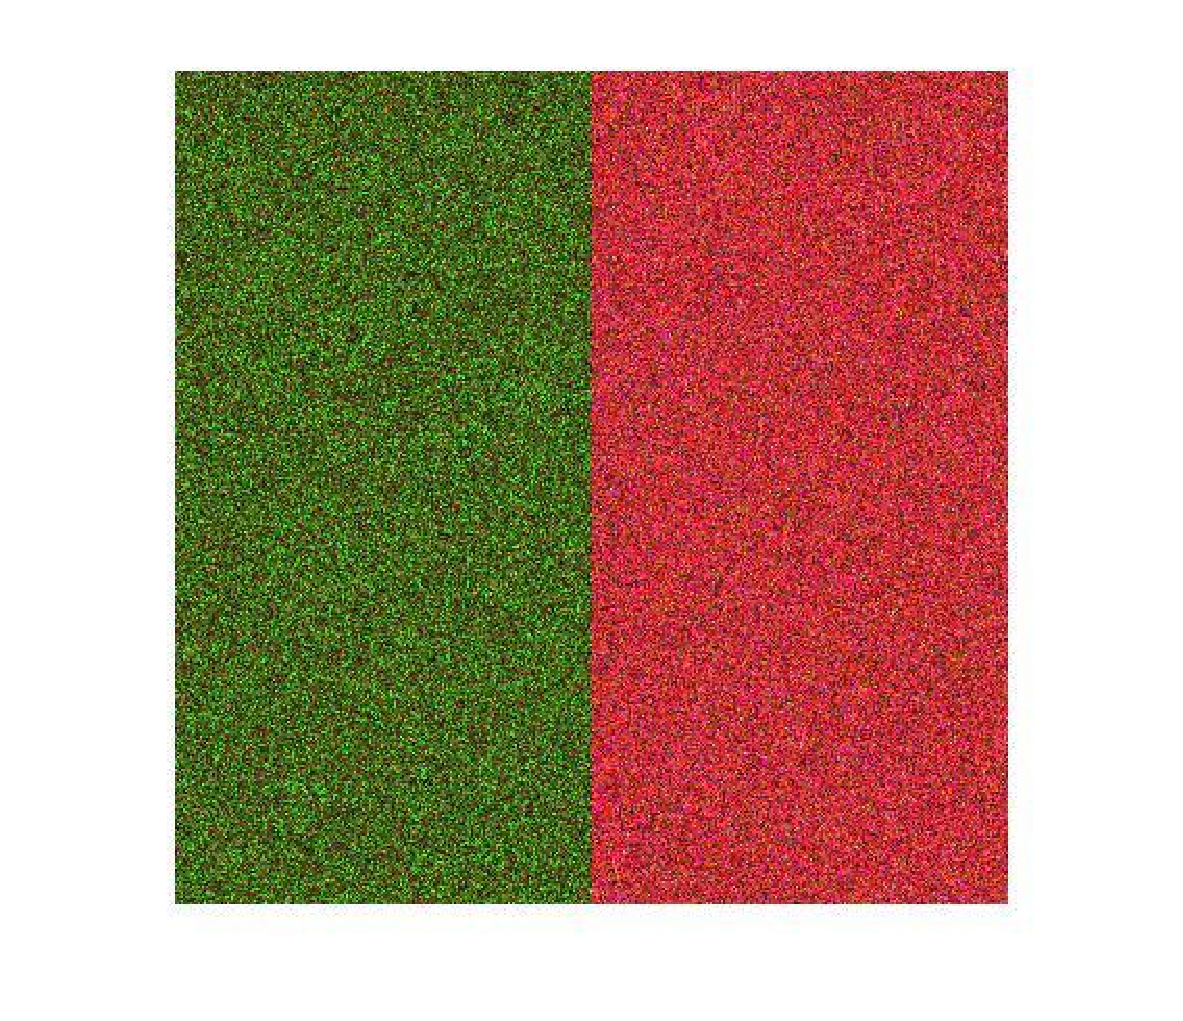
\includegraphics[viewport= 80 50 490 460, clip=true, width=0.23\textwidth]{phanton_nhfc_dec_pauli}}      
     \subfloat[Marginal densities of the $\text{hh}$ channel\label{fig_Edges-Evidence:b}]{%
       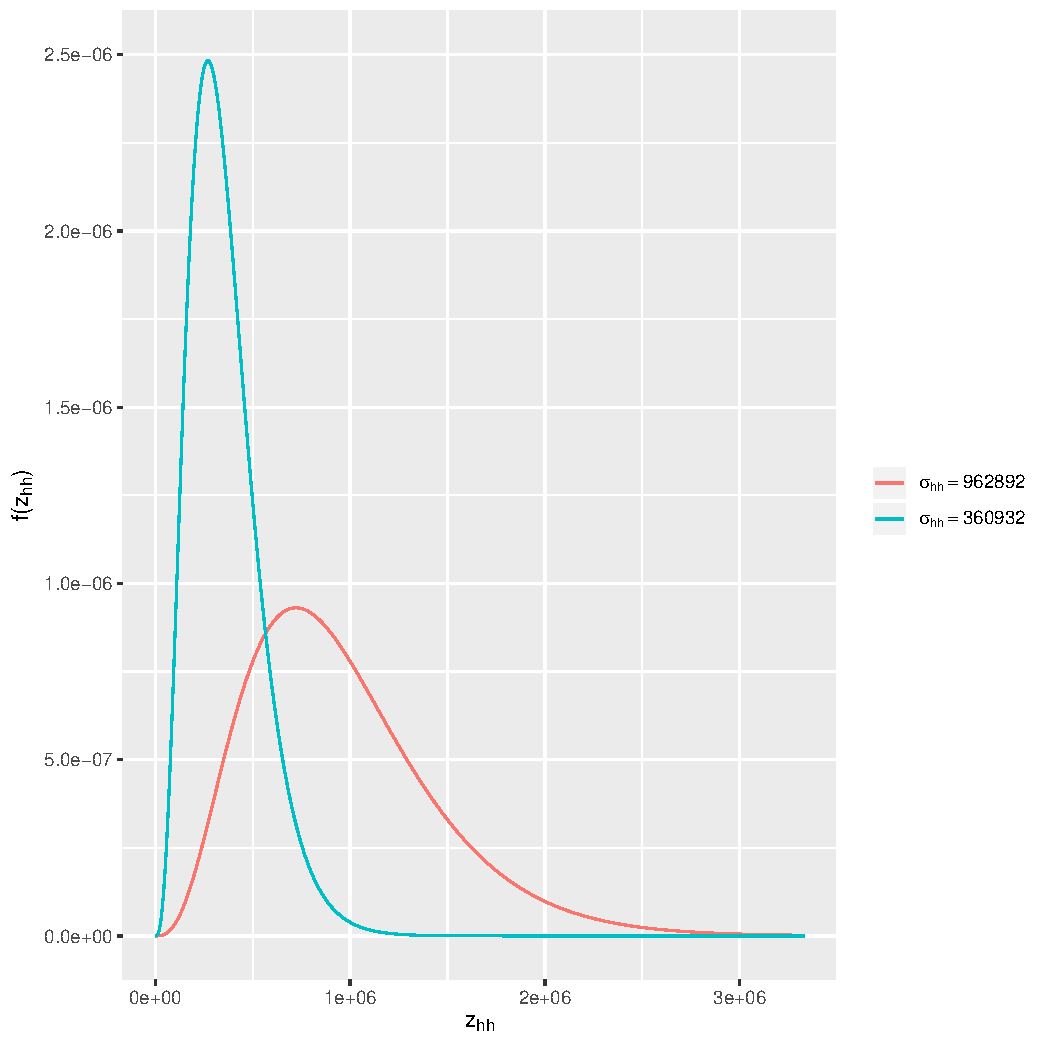
\includegraphics[width=0.24\textwidth]{grafico_pdf_nhfc_2014_sigma_hh_artigos}
     }
    \caption{Edges evidences}
     \label{fig_Edges-Evidence}
\end{figure}
\end{alertblock}
\end{frame}



\begin{frame}[fragile]{PolSAR Image}
\begin{alertblock}{Application in simulated images}
\begin{itemize}
	\item 
	\begin{figure}[hbt]
	\centering
     \subfloat[Channel $\text{hh}$ \label{fig_evid_bordas:1a}]{%
       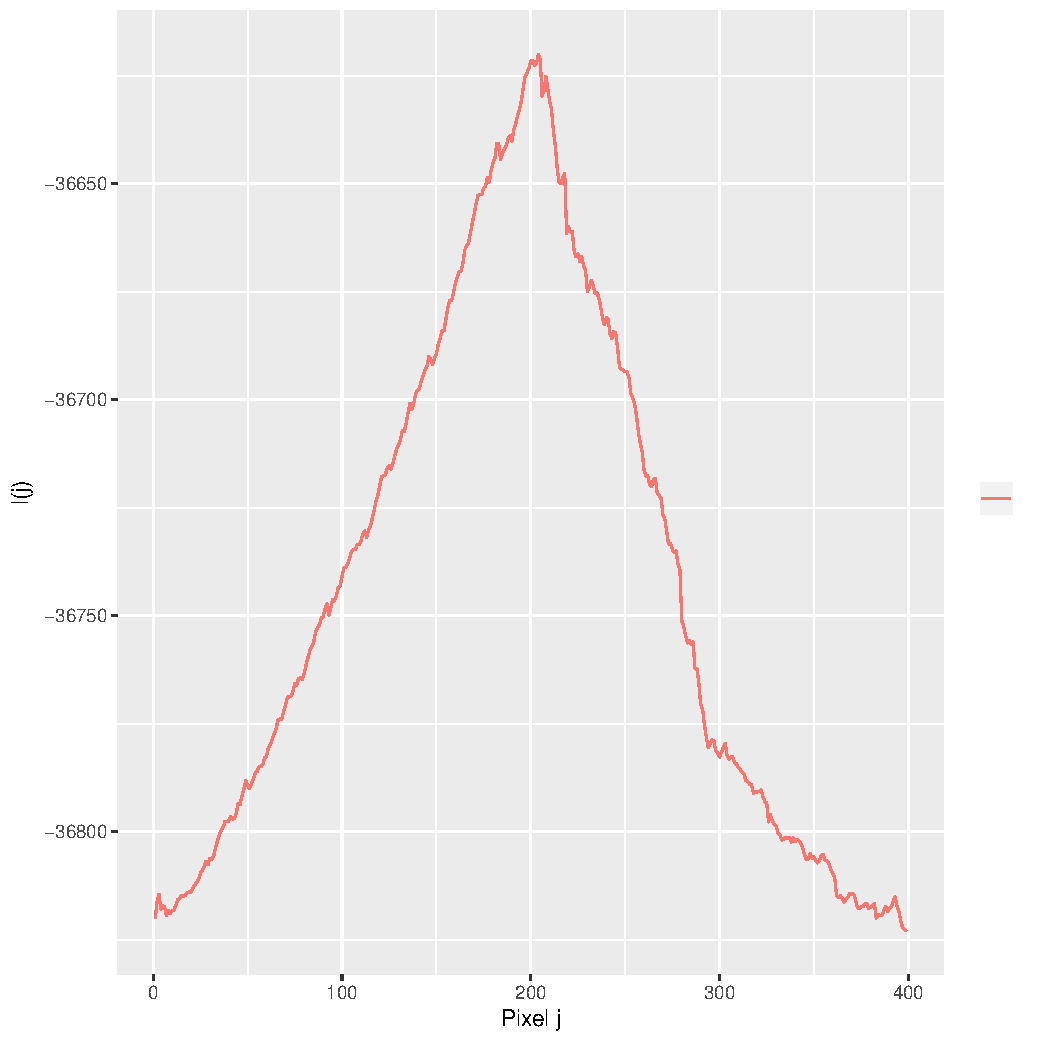
\includegraphics[width=0.32\linewidth]{grafico_l_nhfc_2014_sigmahh_artigos}}
     \subfloat[Channel $\text{hv}$ \label{fig_evid_bordas:1b}]{%
       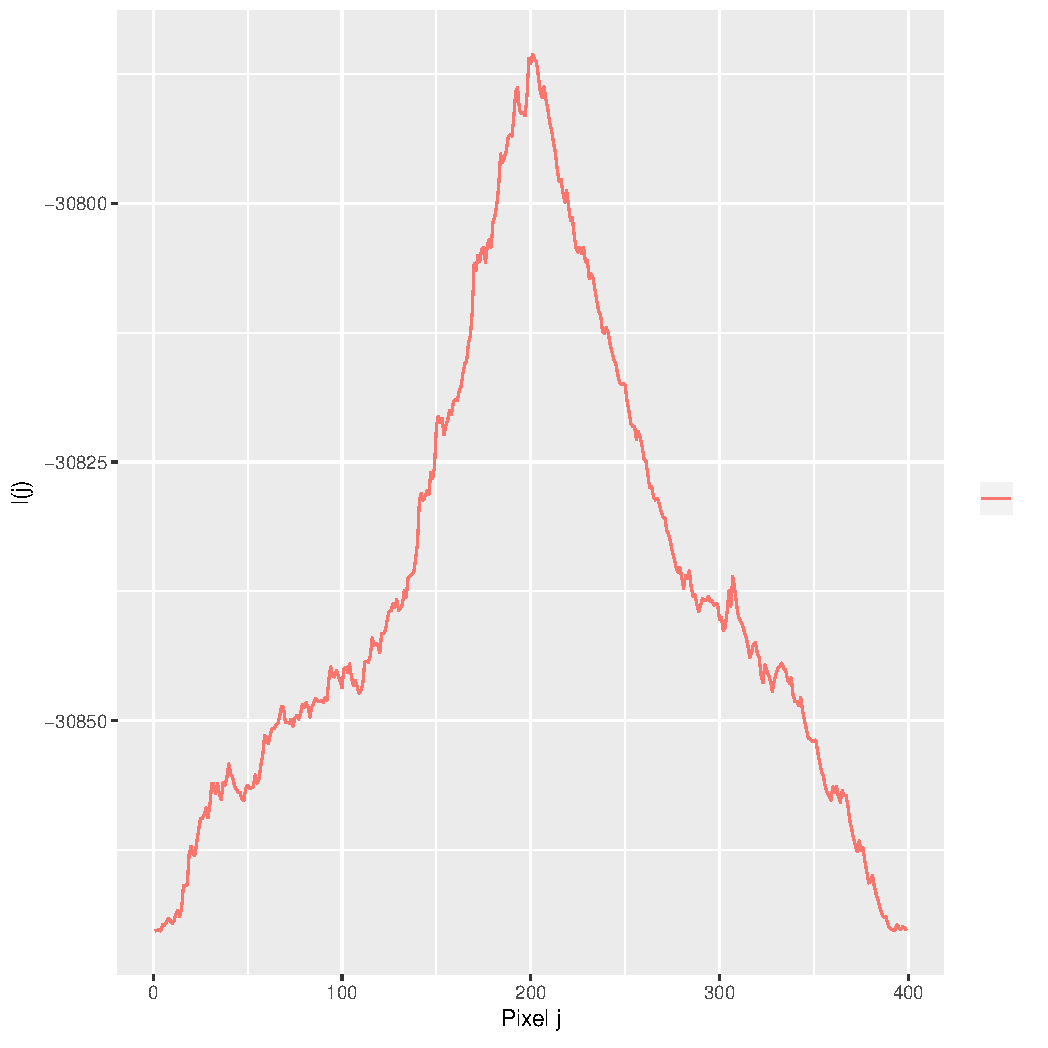
\includegraphics[width=0.32\linewidth]{grafico_l_nhfc_2014_sigmahv_artigos}}
     \subfloat[Channel $\text{vv}$ \label{fig_evid_bordas:1c}]{%
       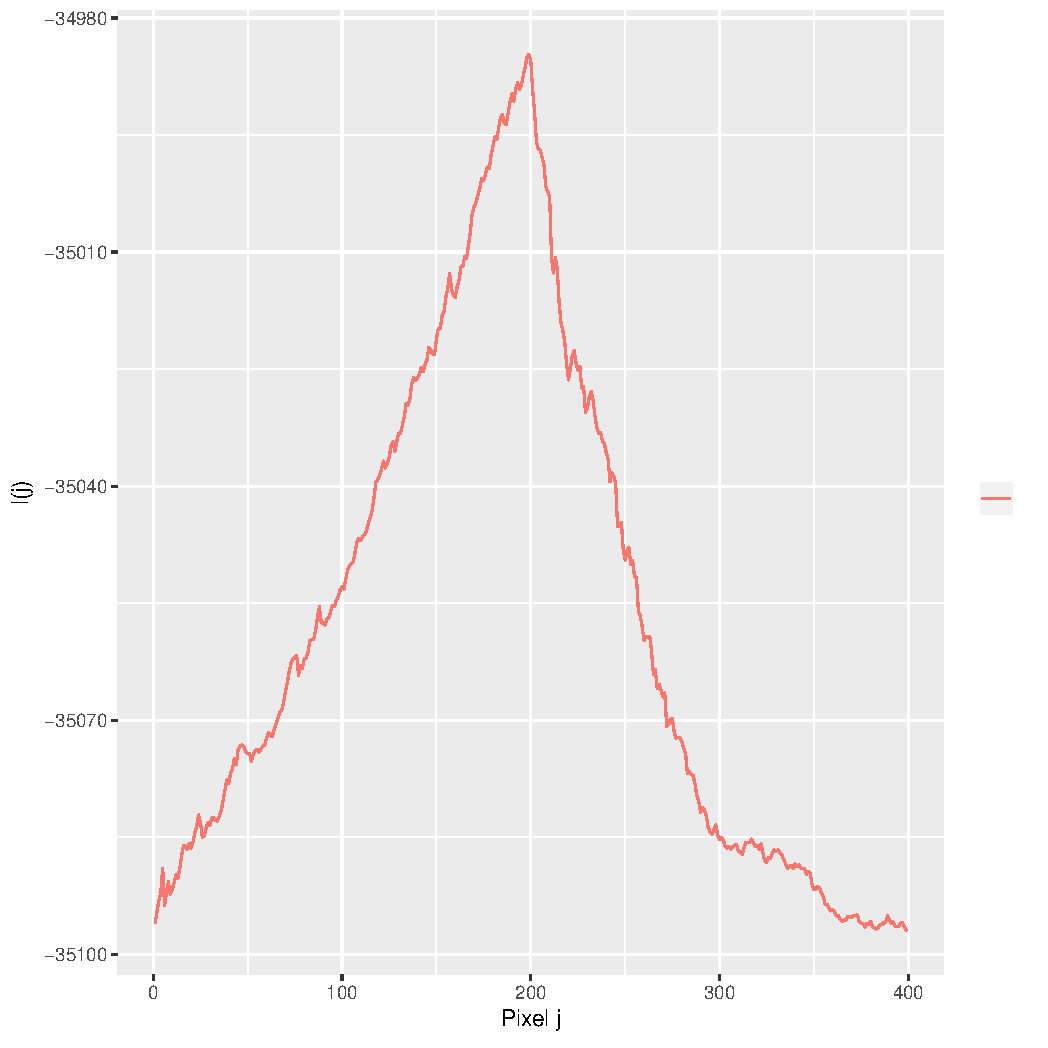
\includegraphics[width=0.32\linewidth]{grafico_l_nhfc_2014_sigmavv_artigos}}
     \caption{Edges evidences}
     \label{fig_evid_bordas}
   \end{figure}	
\end{itemize}
\end{alertblock}
\end{frame}


\begin{frame}[fragile]{PolSAR Image}
\begin{alertblock}{Application in simulated images}
\begin{itemize}
	\item 
	\begin{figure}[hbt]
	\centering
	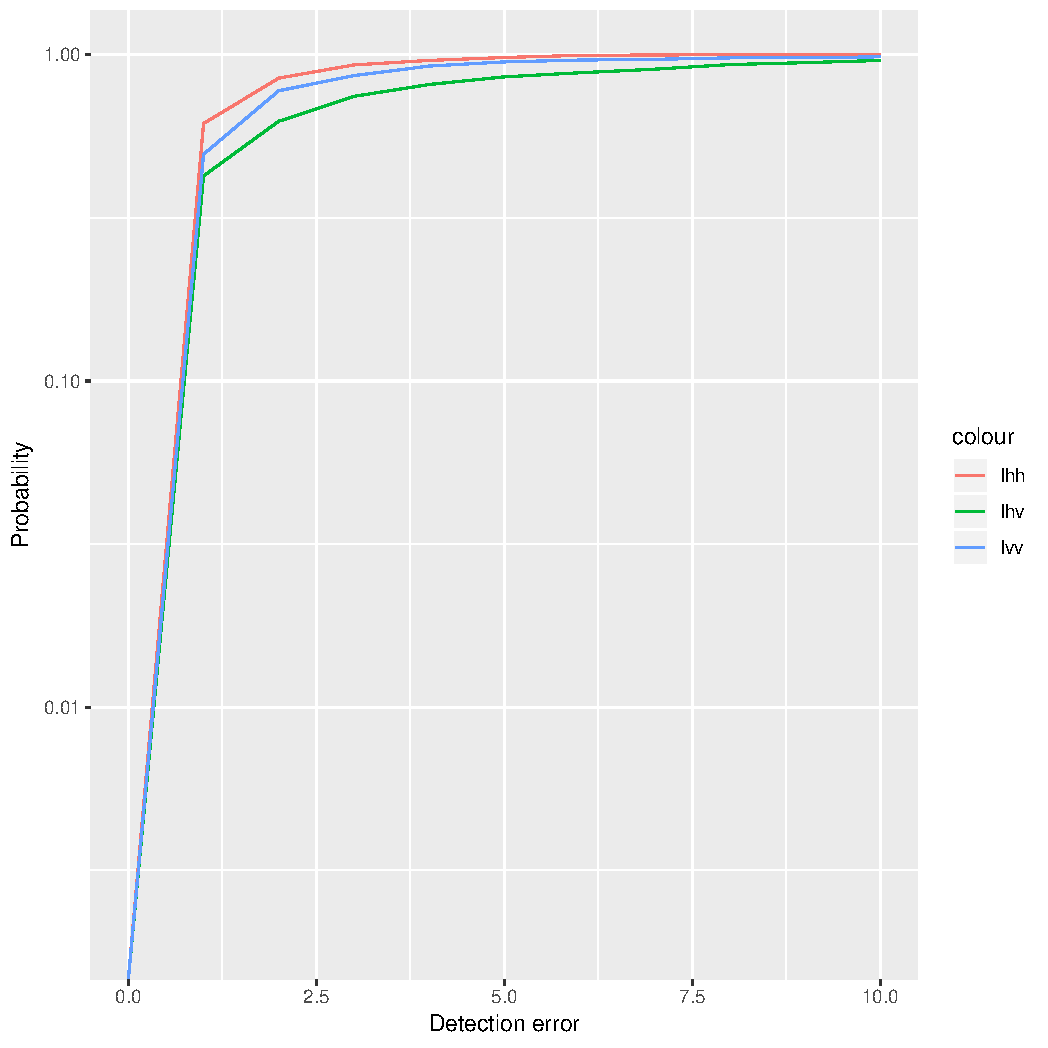
\includegraphics[width=.5\linewidth]{metricas_ihh_ivh_ivv_nhfc_artigos}%
	\caption{Probability of detecting edges evidences.}
\label{probability_edge_detc}
\end{figure}
\end{itemize}
\end{alertblock}
\end{frame}


\begin{frame}[fragile]{PolSAR Image}
\begin{alertblock}{Methods of fusion of edge evidence}
\begin{itemize}
	\item 
	\begin{equation}
	IF(x,y)=\frac{1}{nc}\sum_{i=1}^{nc}IE_i(x,y),
\end{equation} 	
\end{itemize}
\end{alertblock}
\end{frame}


\begin{frame}[fragile]{PolSAR Image}
\begin{alertblock}{Methods of fusion of edge evidence}
\begin{itemize}
	\item Stationary wavelet transform -- SWT
\item  calculate the SWT decomposition by getting $I_\text{HH}$, $I_\text{HL}$, $I_\text{LH}$ and $I_\text{LL}$ for each channel (image);
\item  in the decompositions $I_\text{HH}$, obtain the arithmetic mean of all channels, pixel by pixel. In the decompositions $I_\text{HL}$, $I_\text{LH}$ and $I_\text{LL}$, the maximum between each channel is found, pixel by pixel, leaving a new decomposition $\bar{L}_\text{HH}$, $\bar{I}_\text{HL}$, $\bar{I}_\text{LH}$ and $\bar{I}_\text{LL}$;
\item  perform the inverse SWT transformation. The image is obtained by fusing the edge evidence $IF(x,y)$.  
\end{itemize}
\end{alertblock}
\end{frame}

\begin{frame}[fragile]{PolSAR Image}
\begin{alertblock}{Methods of fusion of edge evidence}
\begin{itemize}
	\item Principal component analysis -- PCA
	\item organize the data in such a way that each image has a column vector, forming a $Y$ matrix of dimension $l\times nc$, where $l=m n$, the lines times the columns of the matrices to be used in the fusion;
\item calculate the average of the elements of these columns, generating a vector dimension of $1\times nc$;
\item subtract the average of each column from the $Y$ matrix, resulting in $X$, a matrix of the same dimension of $Y$; 
\item find $C$, the covariance matrix of $X$;
\item calculate its eigenvalues $\Lambda$ and eigenvectors $D$, and sort the eigenvalues and eigenvectors in descending order. The matrices generated by the eigenvalues, on the main diagonal, and the eigenvectors placed in column, have dimensions $nc\times nc$;
\item compute the components $P_i={V_i}^{-1}{\sum_{i=1}^l V_i}$ with $i=1,\dots,nc$;
\item fuse $IF(x,y)=\sum_{i=1}^{nc}P_iIE_i(x,y)$, recalling that $\sum_{i=1}^{nc}P_i=1$.
\end{itemize}
\end{alertblock}
\end{frame}


\begin{frame}[fragile]{PolSAR Image}
\begin{alertblock}{Methods of fusion of edges evidence}
\begin{itemize}
	\item ROC statistics
	\item[-] obtain the evidence of edges in the channels, and store it in $E_i$ matrices, with $i=1,\dots,nc$ in a binary way;
\item[-] define a $V$ edge frequency matrix. The $V$ matrix is generated by adding the evidence of $E_i$ edges;
\item[-] use thresholds ranging from $t=1,\dots,nc$ generating $M_t$ matrices;
\item[-] compare each $M_t$, fixed with all $E_i$, find the confusion matrix to generate the ROC curve. The point of the ROC curve closest (in the sense of the Euclidean distance) to the diagnostic line will have its threshold considered optimal;
\item[-] the $M_t$ matrix which corresponds to the threshold closest to the diagnostic line is the result of the fusion.
\end{itemize}
\end{alertblock}
\end{frame}

\begin{frame}[fragile]{PolSAR Image}
\begin{alertblock}{Numerical results}
\begin{itemize}
	\item 
	\begin{figure}[hbt]
\centering
	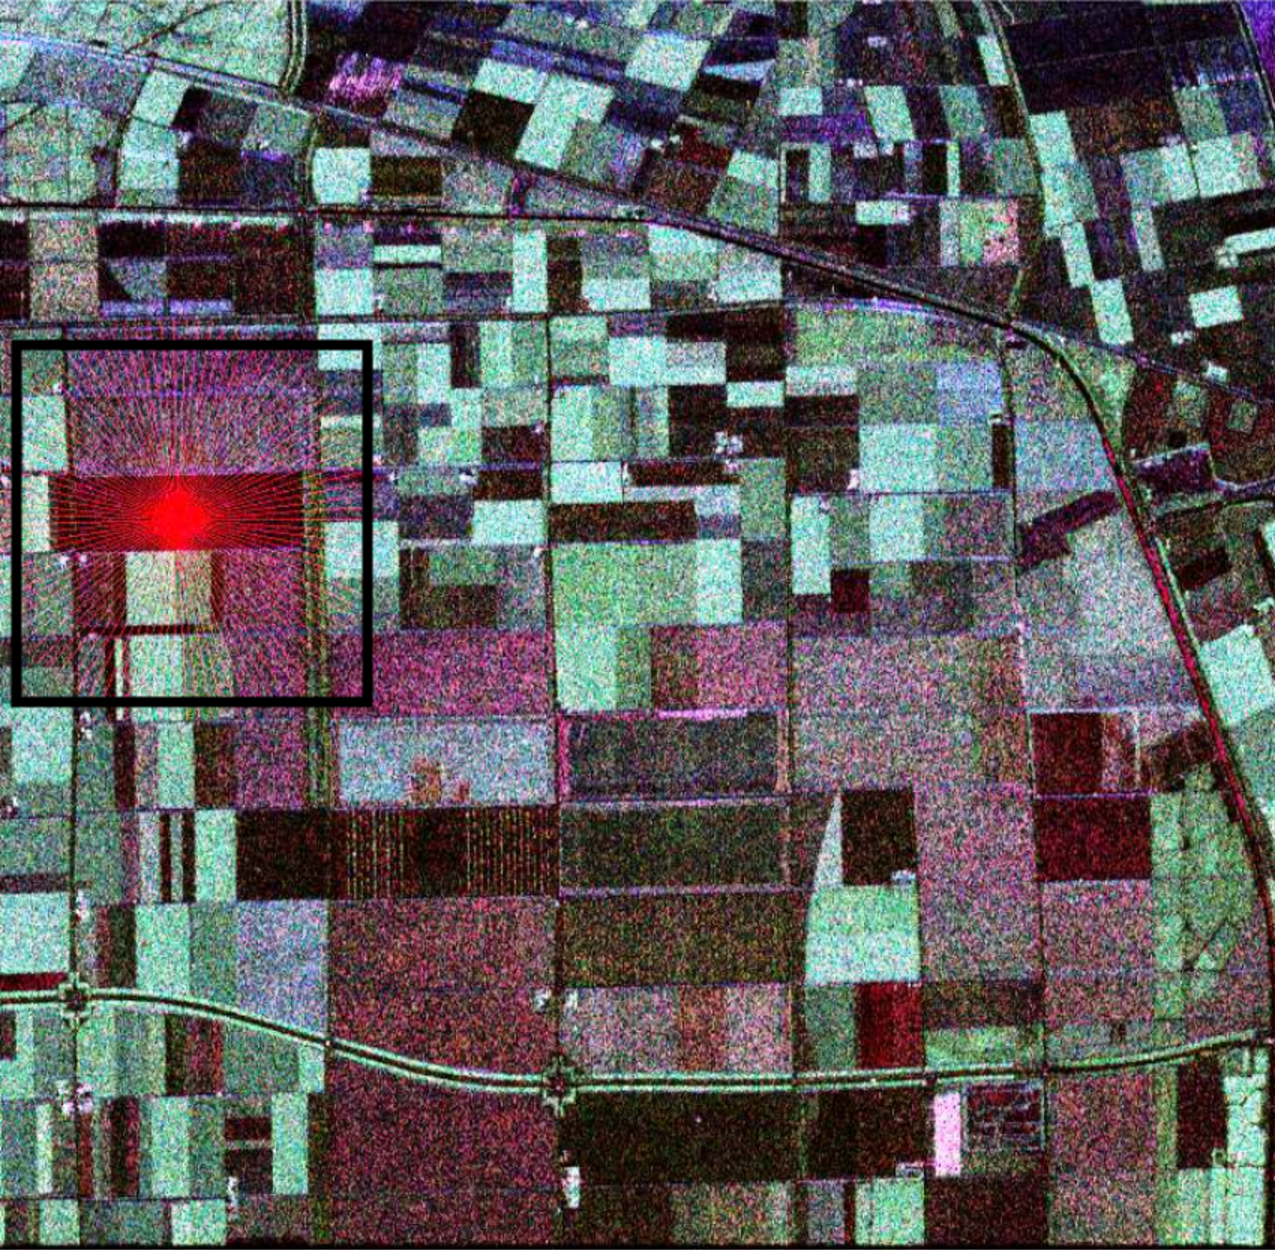
\includegraphics[width=.5\linewidth]{flevoland_radial_4_look_black}
	\caption{Region of interest (ROI) in the image of Flevoland.}
\label{flevoland_radial_4look}
\end{figure}
\end{itemize}
\end{alertblock}
\end{frame}

\begin{frame}[fragile]{PolSAR Image}
\begin{alertblock}{Numerical results}
\begin{itemize}
	\item 
	\begin{figure}[hbt]
	\centering
     \subfloat[Evidences in channel $\text{hh}$ \label{evidencias_hh_hv_vv:a}]{%
       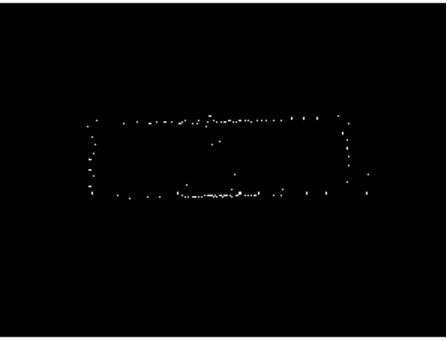
\includegraphics[width=0.32\linewidth]{flevoland_hh_evid_crop_teste}
     }
     \subfloat[Evidences in channel $\text{hv}$ \label{evidencias_hh_hv_vv:b}]{%
       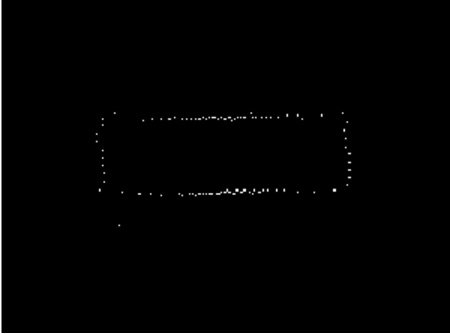
\includegraphics[width=0.32\linewidth]{flevoland_hv_evid_crop_teste}
     }
     \subfloat[Evidences in channel $\text{vv}$ \label{evidencias_hh_hv_vv:c}]{%
       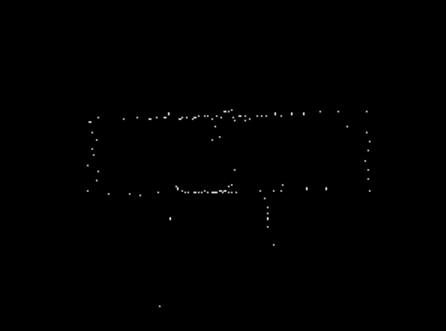
\includegraphics[width=0.32\linewidth]{flevoland_vv_evid_crop_teste}
     }
     \caption{Edges evidences}
     \label{evidencias_hh_hv_vv}
   \end{figure}	
\end{itemize}
\end{alertblock}
\end{frame}

\begin{frame}[fragile]{PolSAR Image}
\begin{alertblock}{Methods of fusion of edge evidence}
\begin{itemize}
	\item \begin{figure}[hbt]
	\centering
     \subfloat[Average fusion\label{fusion_met:a}]{%
       %\includegraphics[width=0.2\textwidth]{example-image-a}
       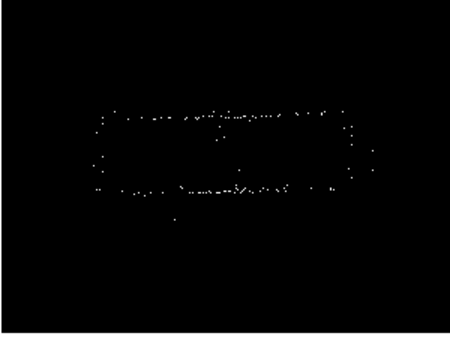
\includegraphics[width=0.32\linewidth]{flevoland_fusao_media_crop_teste}
     }
     \subfloat[SWT fusion\label{fusion_met:b}]{%
       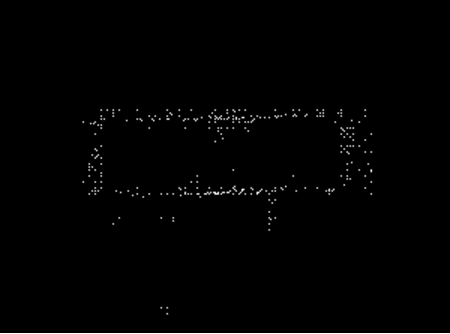
\includegraphics[width=0.32\linewidth]{flevoland_fusao_swt_crop_teste}
     }
     \subfloat[PCA fusion \label{fusion_met:c}]{%
       %\includegraphics[width=0.2\textwidth]{example-image-a}
       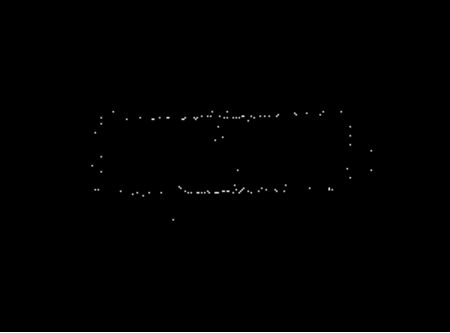
\includegraphics[width=0.32\linewidth]{flevoland_fusao_pca_crop_teste}       
     }\\
     \subfloat[ROC fusion\label{fusion_met:d}]{%
       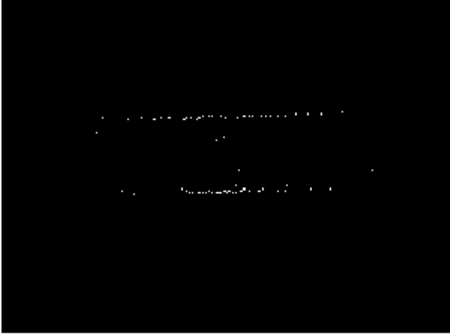
\includegraphics[width=0.32\linewidth]{flevoland_fusao_roc_crop_teste.pdf}
     }
     \caption{Fusion methods}
     \label{fusion_met}
\end{figure}
\end{itemize}
\end{alertblock}
\end{frame}

\begin{frame}[fragile]{PolSAR Image}
\begin{alertblock}{Conclusion}
\begin{itemize}
	\item 
\end{itemize}
\end{alertblock}
\end{frame}


\begin{frame}[allowframebreaks]
\bibliographystyle{IEEEtran}
\bibliography{../bibliografia}
\end{frame}

\end{document}
